\chapter{Einführung in Reactive Programming mit RxJava2}\label{rp_einfuehrung}
Der zentrale Baustein dieser Bibliothek ist die Observable-Klasse im Zusammenspiel mit dem Observer Interface. Ein Observable repräsentiert einen Data- beziehungsweise Eventstream. Es ist für das Push-Verfahren konzipiert (reaktiv) kann aber auch mit dem Pull-Vorgehen verwendet werden (interaktiv)\footnote{Vgl. \cite{Nurkiewicz.2017}, Seite 4.}. Weitere Eigenschaften sind die Nutzung für asynchrone und synchrone Implementierungen und die Repräsentation von Null bis unendliche\footnote{Mathematisch gesehen: $D = [0, \infty)$} viele Werte oder Ereignisse im Laufe der Zeit. Es folgt nun eine kurze Schilderung wie diese Eigenschaften erreicht werden bevor die eigentlichen Struktur, im Genauen eine Beschreibung der Basisklassen, der Bibliothek veranschaulicht wird. Diese Eigenschaften wurden vom bereits erwähnten Ben Christensen in Kapitel 1 innerhalb des Buches von Tomasz Nurkiewicz \footnote{\cite{Nurkiewicz.2017}} beschrieben.
\section{Synchronität und Asynchronität}
Bei dem bisher gelesenen wird schnell klar, dass die Asynchronität ein essentieller Bestandteil sein muss. Jedoch ist das Observable standardmäßig synchron implementiert und ein asynchrones Verhalten muss explizit gefordert werden. Erfolg eine Subscription eines Observers an einem Observable wird die Weitergabe der Elemente des Streams auf dem Thread des Observers ausgeführt. Ebenso finden die Bulk Operations, also Transformation, Modifikation und Komposition der Elemente oder Streams grundsätzlich synchron statt. Werden also Daten zum Beispiel aus einem Cache geladen und über den Stream zur Verfügung gestellt ist der Standardweg des synchronen Vorgehens vollkommen richtig um den Overhead der expliziten Asynchronität zu umgehen. Finden aber Abfragen zum Beispiel über eine Netzwerkressource statt, die unterschiedliche lange Latenzen aufweist, kann es notwendig sein die Anfragen auf weiteren Threads auszuführen. Dies kann mittels eigens erstellte Threads, Threadpools oder Schedulers umgesetzt werden. Somit werden die Callback Methoden des Observers von dem zusätzlichen erstellten Thread aufgerufen und der eigentliche Observer Thread wird nicht weiter blockiert.
\section{Parallelisierung und Nebenläufigkeit}
Wie bekannt sein dürfte ist die Parallelisierung und Nebenläufigkeit eher auf Systemebene zu betrachten. Als parallel bezeichnet man die Ausführung unterschiedlicher Tasks auf verschiedenen Kernen oder Maschinen. Voraussetzung ist die wirklich gleichzeitige Bearbeitung der Tasks. Von Nebenläufigkeit wird gesprochen wenn eine Recheneinheit mehre Tasks oder Threads verarbeitet und immer nur einer dieser Aufgaben zur einer Zeit bearbeitet wird. Nach einem gewissen Zeitraum bekommt ein anderen Task die Rechenleistung und die vorherige Task wurde beendet wenn die Aufgabe erfüllt wurde oder wartet auf erneute Rechenzeit. Dieses Verfahren wird \textit{time slicing} genannt und wird von Kernel des Betriebssystems verwaltet. Somit ist Parallelisierung immer auch nebenläufig aber Nebenläufigkeit nicht unbedingt auch parallelisiert. Um dieses Verfahren in Verbindung mit den Observables zu bringen ist zu sagen, dass ein Observable Objekt immer serialisiert und thread-safe sein muss. Die Callback-Methoden des Subscribers dürfen also nie zeitgleich aufgerufen werden. Parallelisierung und Nebenläufigkeit werden also dadurch erreicht, dass man Observables miteinander verbindet und jeder der Streams parallel oder nebenläufig mit den jeweils anderen interagieren kann zum Beispiel mit den Bulk-Operations merge und zip, aber dazu später mehr.
\section{Push und Pull}
Wird synchrones Pulling von Objekten einer Liste über das Iterable Interface durchgeführt, so wird im Gegenzug ein asynchrones Pushing via Observable realisiert. Beide Schnittstellen bieten die gleiche Funktionalität nur der Datenfluss findet in die entgegengesetzte Richtung statt. Durch diese Dualität können beide Vorgehen äquivalent verwendet werden. Will man ein weiteres Objekt einer Liste über den Iterator abfragen, wird die next()-Methode aktiv aufgerufen und wenn vorhanden wird ein weiteres Objekt dem Verbraucher zurück gegeben. Hingegen wird bei der Verwendung von Observables die Daten des Streams mit der onNext()-Methode\footnote{Diese Methode wird durch ein Autftreten eines Ereignisses oder von Daten im Stream aufgerufen. Somit handelt es sich bei dieser Art Methode um Callback Methoden.} des Verbrauchers gepusht. Wie die Tabelle \ref{tbl:vglIterObs}\footnote{Quelle: \cite{reactivex.io}} zeigt gilt dies ebenso beim Auftreten eines Fehlers oder beim Erreichen des Endes der Datenquelle.
\begin{table}[]
	\centering
	\begin{tabular}{|c|c|lll}
		\cline{1-2}
		\cellcolor[HTML]{C0C0C0}Pull (Iterable) & \cellcolor[HTML]{C0C0C0}Push (Observable) &  &  &  \\ \cline{1-2}
		T next()                                & onNext(T)                                 &  &  &  \\ \cline{1-2}
		throws Exception                        & onError(Throwable)                        &  &  &  \\ \cline{1-2}
		returns                                 & onComplete()                             &  &  &  \\ \cline{1-2}
	\end{tabular}
	\caption{Vergleich zwischen Funktionalität der Iterable- und Observable-Schnittstelle}
	\label{tbl:vglIterObs}
\end{table}
Die Verbindung zwischen Observable und Observer findet über ein Subscription statt. Damit werden die beiden zu einem Paar gebunden und die entsprechenden Methoden des Observers können nun von dem Stream angesprochen werden. Dies beschreibt auch noch eine weitere Eigenschaft. Ein Observable publiziert nur die Ereignisse wenn es jemanden gibt der diese Ereignisse auch fordert. Dies wird auch als \textit{faules} Verhalten bezeichnet. Somit wird das Arbeiten durch das Subscriben und nicht durch das Erstellen eines Observables verursacht. Im Vergleich dazu kann ein Objekt vom Typ Future betrachtet werden. Wird ein Future erstellt, wird auf ein Ergebnis gewartet, welches direkt und einmalig asynchron ausgeführt wird und innerhalb des Futures zur Verfügung steht sobald das Ereignis abgeschlossen ist. Ein mehrfaches Ausführen eines Futures ist nicht möglich, anders als beim Observable wo zu jeder Zeit ein weiterer Subscriber hinzu kommen kann. Somit ist ein Observable-Objekt beliebig oft verwendbar. 
\section{Observable}
Es wurde in den vorherigen Abschnitten schon etwas über das Observable gesagt, doch der Vollständigkeit halber wird hier seine Eigenschaften und Fähigkeiten zusammengefasst beschrieben. Es handelt sich hierbei um die Quintessenz der RxJava Bibliothek.
\lstinputlisting[linerange={7-13}, caption={Beispiel Observable Initialisierung und Subscription}, label=lst:obsexample]{../SystemMonitor/examples/obs/ObservableExample.java}
Der Ereignisstrom über einen Zeitraum wird von dem Observable repräsentiert. Dieser Ereignisstrom ist jedoch variabel. Weder muss die Anzahl der auftretenden Ereignisse bekannt sein, noch müssen diese in einem geregelten Intervall auftreten. Ebenso wenig muss der Zeitraum begrenzt sein, was bedeutet, dass es sich auch im unendliche Eventstreams handelt kann. Die Tabelle \ref{tbl:vglIterObs} zeigt die Methodenaufrufe die eine Observable auslösen kann. Somit wird auch klar, dass nur drei Arten von Events auftreten können. Eine beliebige Anzahl von \textit{onNext(T)}-Methodenaufrufen mit dem Eventtyp T, das einmalige Event der Fertigstellung mit dem \textit{onComplete()}-Aufruf oder das Aufkommen eines Fehlers wird kommuniziert mit der \textit{onError(Throwable)}-Methode. Somit gilt: 
\begin{displaymath}
	OnNext\cdot(OnComplete | OnError)?
\end{displaymath}
Daraus resultiert das entweder ein gewolltes Ende oder ein unvorhergesehener Fehler auftritt, aber niemals beides\footnote{pdf in bib aufnehmen und zum regex binden}. Schaut man sich nun Listing \ref{lst:obsexample} an, sieht man den Ablauf. Ein Observable wird initialisiert\footnote{Es gibt unterschiedliche Methoden je nach Objektart welche als Observable dargestellt werden soll. Eine Liste finden man hier: https://github.com/ReactiveX/RxJava/wiki/Creating-Observables}, hier mit drei Elementen, also ein endlicher Stream. Durch das \textit{subscribe} wird anonym ein Subscriber beschrieben. Bei dem ersten Lambda-Ausdruck handelt es sich um die \textit{onNext()}-Methode. Weiter geht es mit \textit{onError()} und \textit{onComplete()}. Man sieht bei einem fehlerfreien Durchlauf die drei Elemente auf der Konsole und ebenso die Ausgabe für das beenden des Streams. Würde ein Fehler auftreten würde die Ausgabe der Elemente beendet werden und der Stacktrace würde ausgegeben werden, statt des \textit{finish}-Strings. Auch wurde schon ein wichtiger Punkt angeschnitten, nämlich dass zu jeder Zeit ein neuer Subscriber hinzu kommen kann. Jeder Subscriber erhält seine eigene Kopie die Streams. Dies nennt man auch \textit{Cold Observable}.
\lstinputlisting[linerange={12-17}, caption={Beispiel Cold Observable}, label=lst:coldobs]{../SystemMonitor/examples/hotandcold/HotAndCold.java}
Wie hier in Listing \ref{lst:coldobs} zu sehen werden zwei Kopien des Observable-Streams erstellt. Es ist zu beachten, dass somit jeder Subscriber einen eigenen Timer bekommt. Will man nun aber die beiden Rechenoperation immer auf den selben Wert durchführen wird es auf diesem Wege nicht funktionieren. Somit muss es die Möglichkeit geben diese Informationen zu teilen.
\lstinputlisting[linerange={20-25}, caption={Beispiel Hot Observable}, label=lst:hotobs]{../SystemMonitor/examples/hotandcold/HotAndCold.java}
Der Methodenaufruf \textit{publish()} ist hier der Schlüssel. In Listing \ref{lst:hotobs} sieht man, nachdem das Intervall gestartet wird besagten Aufruf. Sollen Daten geteilt werden spricht man von einem \textit{Hot Observable}. Via \textit{publish()} erfährt das Observable-Objekt, dass die Daten geteilt werden sollen. Mit \textit{autoConnect()} wird bestätigt, dass sich jeder neue Subscriber automatisch verbinden kann. Als Parameter kann auch eine Begrenzung für die Subscriber-Anzahl übergeben werden. Grundlegend hat sich am Aufbau des Observerables nichts geändert. Sobald ein Hot Observable eine Subscription erhält beginnt es Daten auszugeben. Schaltet sich nun ein weiterer Subscriber auf den Stream beginnt er mit den Werten die auch der oder die anderen Subscriber erhalten. Somit wird der neue Subscriber die schon vergangenen Events nicht mehr erfahren können. Es macht zum Beispiel Sinn, wenn eine Mausbewegung getrackt wird, da neue Subscriber nicht wissen müssen wo sich der Mauszeiger vorher befand, sondern es ist nur wichtig wo sich der Zeiger aktuell befindet. Je nach Problemstellung ist das eine oder das andere von Vorteil. Ist es entscheidend eine konsistente und vollständige Abarbeitung von Events durchzuführen geht kein Weg an Cold Observables vorbei. Handelt es sich um einen Stream über den man keine konkrete Kontrolle hat, Paradebeispiel I/O, wird man meist auf Hot Observables zurück greifen. \\ Es gibt eine Unzahl an Methoden und vor allen Dingen Bulk Operations die auf einem Observable Stream ausgeführt werden können. Die komplette Übersicht findet man in der Javadoc\footnote{Vgl. \cite{rx.javadoc}}. Ein Punkt welcher das Observable nicht abdeckt ist das Back Pressure. Es sind keine Möglichkeiten erhalten die auf Back Pressure reagieren können. Jedoch ist nicht blockierender Back Pressure ja notwendig um mit der Reactive Streams Initative konform zu gehen. Daher wurde die Klasse \textit{Flowable} implementiert.
\section{Flowable}
Diese Klasse ist nach den Kriterien der Reactive Streams realisiert. Flowable bietet weitestgehend alles, was auch Observable zu bieten hat, bringt aber durch die Implementierung \textit{"implements org.reactivestreams.Publisher<T>"} des Publisher Interfaces eine  hervorragende Verträglichkeit zu den Reactive Streams mit sich. Ebenso besteht die Möglichkeit Back Pressure zu handhaben, indem Puffergrößen\footnote{Flowable.observeOn hat standardmäßig Platz für 128 Elemente im Puffer} eingestellt werden können\footnote{Beispiel für Buffer settings von flowable}. In der offiziellen Dokumentation von RxJava2\footnote{Vgl.https://github.com/ReactiveX/RxJava/wiki/What's-different-in-2.0} wird beschrieben wann es sich besser eignet auf Observable oder aber auf Flowable zu setzt. \\ \underline{Wann sollte man Observable nutzen:}
\begin{itemize}
	\item Wenn im Datenfluss nicht mehr als 1000 Elemente auftreten, es somit als keine Chance für einen \textit{OutOfMemoryError} gibt.
	\item Wenn GUI Events behandelt werden. Diese können nicht durch ihr unregelmäßiges Aufkommen schlecht gepuffert werden. Außerdem ist das Auftreten meist geringfügig. Elemente in der Auftrittshäufigkeit von maximal 1000 Hz sollte zu bewältigen sein.
	\item Wenn die Plattform keine Streams unterstützt, also die Java Version diese noch nicht bereit stellt. Grundsätzlich bringen Observables weniger Overhead mit sich.
\end{itemize}
\underline{Wann sollte man Flowable nutzen:}
\begin{itemize}
	\item Wenn mehrere Tausende Elemente generiert werden und die Möglichkeit vorhanden ist mit der Quelle zu kommunizieren um bei fehlendem Back Pressure die Frequenz zu regeln.
	\item Beim Lesen von der Festplatte. Dies geschieht blockierend und mit dem Pull-Ansatz, was sich hervorragend eignet um die Elemente als Back Pressure zu puffern.
	\item Beim Lesen aus der Datenbank. Auch das geschieht via Pull und blockiert. Also wieder von Vorteil mit einem Puffer zu arbeiten.
	\item Kommunikation über ein Netzwerk. Hierbei kann, sofern unterstützt, eine logische Menge an Elementen angefragt werden welche im Puffer gesichert werden und nach und nach abgearbeitet werden können.
	\item Weiter blockierende auf Pull-basierenden Datenquellen deren API eventuell in Zukunft auch auf ein reaktives Verhalten umgestellt werden. Hier liegt der Vorteil in der Reactive Streams Konvention die auch in Zukunft verwendet werden wird.
\end{itemize}
Betrachtet man das Listing \ref{lst:flowexample} sieht man im Vergleich zum Observable den Aufruf der \textit{onBackpressureBuffer()}-Methode. Hiermit kann direkt eine Puffergröße für jede Subscription festgelegt werden. 
\lstinputlisting[linerange={7-13}, caption={Beispiel Flowable mit Back Pressure}, label=lst:flowexample]{../SystemMonitor/examples/flow/FlowExample.java}
\section{Single}
Wo Observable oder Flow eine Menge von Null bis endliche viele Elemente ausgeben, steht Singe, wie der Name schon sagt, dafür, dass immer nur ein Wert ausgegeben wird. Somit sind auch die drei bekannten Methoden zur Datenausgabe hier überflüssig. Stattdessen sind nur zwei Methoden vorhanden, \textit{onSuccess()} und \textit{onError()}. Auch hier gilt das immer nur eine der Methoden aufgerufen werden kann. Also eine erfolgreiche Datenausgabe oder eine fehlerbehaftete. Anschließend werden die Subscriptions gelöst und das Singe wird beendet. Auch hier sind wieder eine Reihe von Bulk Operation möglich. 
\lstinputlisting[linerange={7-14}, caption={Beispiel eines Singles}, label=lst:singleexample]{../SystemMonitor/examples/single/SingleExample.java}
In Listing \ref{lst:singleexample} sieht man die Verwendung eines Single-Objekts. Es kann nur mit einem Objekt erstellt werden, di Bearbeitung dieses Elements findet wieder mit einer Auswahl an bekannten Operation statt. In der \textit{subscribe()}-Methode sieht man die zwei Lambda-Ausdrücke die wieder die möglichen Methodenaufrufe, also bei Erfolg oder Fehlerfall, die ausgeführt werden können.
\section{Subject}
Also Subject versteht man ein Objekt, dass sowohl als Observable und auch als Observer fungieren kann. Es kann an mehreren Observables subscriben, diese Daten verarbeiten und seinen eigenen Subscribern weiterleiten. 
\lstinputlisting[linerange={7-14}, caption={Beispielverwendung eines Subjects}, label=lst:subjectexample]{../SystemMonitor/examples/subject/SubjectExample.java}
Um es das Vorgehen bei Verwendung eines Subject zu veranschaulichen betracheten wir Listing \ref{lst:subjectexample}. Wir erstellen wieder das schon bekannte Observable-Objekt und ein Subject, hier ein speziell ein PublicSubject. Dieses Subject bekommt eine Subscription in welcher alle String-Werte in Großbuchstaben umgewandelt und anschließen auf der Konsole geschrieben werden. Wenn nun das Subject selbst an dem vorhanden Observable subscribed, werden die von diesem ausgegebenen Werte an gemapped und an die Subscription des Subject weitergegeben. Zusätzlich zum PublicSubject stehen noch drei weitere Arten zur Verwendung bereit:
\begin{itemize}
	\item \underline{AsycSubject:} Ein AsyncSubject gibt seinen Subscribern nur den letzte Wert der Quelle weiter, und das auch nur falls das Quell-Observable beendet wurde. Endet es durch einen Fehler wird die Fehlermeldung direkt an die Subscriber des Subjects weiter gereicht.
	\item \underline{BehaviorSubject:} Ein BehaviorSubject beginnt sobald es einen Subscriber verzeichnet kann mit der Übermittlung des letzten Wertes der Quelle, oder mit einem Standardwert falls von der Quelle noch nichts ausgegeben wurde. Anschließend werden alle weiteren Werte weitergegeben. Auch hier wird bei Auftreten einen Fehler die Meldung direkt durchgereicht.
	\item \underline{PublishSubject:} Ein PublishSubject überträgt genau die Werte, die von seiner Quelle in dem Zeitraum, in welchem auch eine Subscription vorliegt, ausgegeben wurden. Alles vorherige wird nicht übermittelt. Somit liegt ein Verhalten eines Hot-Observables vor.
	\item \underline{ReplaySubject:} Ein ReplaySubject überträgt an jeden Subscriber alle Werte die jemals von seiner Quelle ausgegeben wurden. Dies ist mit Vorsicht zu genießen da hier natürlich ein Back Pressure Problem nahe liegt. 
\end{itemize}
Dieses Back Pressure Problem kann wie schon beim Observable nicht direkt gelöst werden. Somit ist auch hier noch keine Konformität zur Reactive Streams Initiative zu sehen. Dafür gibt es eine weiter Klasse: die Processor-Klasse.
\section{Processor}
Was das Flowable für das Observable ist, stellt der Processor für das Subject dar. Eine Implementierung um den Anforderungen der Reactive Streams gerecht zu werden. Die Kompatibilität und das Handling des Back Pressures stehen auch hier wieder im Vordergrund. Die vier Ausprägungen des Subject sind auch bei der Processor-Klasse wiederzufinden. Zusätzlich wurde noch der \textit{UnicastProcessor} implementiert. Hier wird nur genau ein Subscriber zugelassen über die komplette Existenz des Processor-Objekts. Wenn versucht wird dagegen zu verstoßen wird eine \textit{IllegalStateException} geworfen.
\lstinputlisting[linerange={7-15}, caption={Beispielverwendung eines Processors}, label=lst:processorexample]{../SystemMonitor/examples/processor/ProcessorExample.java}
In Listing \ref{lst:processorexample} ist ein einfaches Beispiel zu finden. Die Ähnlichkeit zur Subject-Klasse ist unverkennbar. Jedoch werden hier eben die Flowables verwendet, und das Back Pressure kann kontrolliert werden. Ist also bekannt das Schnittstellen nach den Richtlinien der Reactive Streams Initiative entwickelt wurden, ist es lohnenswert auf die Verwendung von Flowables und Processors zu setzten um auf einfachem Wege eine Kompatibilität zu ermöglichen.
\section{Schedulers}
Im Abschnitt zu Parallelisierung und Nebenläufigkeit wurde schon beschrieben, dass jedes Observable-Objekt serialisierbar und thread-safe gestaltet wird. Auch Threads kamen zur Sprache und wie eine Parallelisierung oder Nebenläufigkeit erozeugt werden kann. Da jeder der Bulk Operations auf einem Observable immer wieder ein neues, eigenständiges Observable weiterreicht, besteht die Möglichkeit Verarbeitungsschritte auf anderen Threads als auf dem des Subscribers auszuführen. Dafür bringt das Observable zwei Operationen mit, \textit{subscribeOn} und \textit{observeOn}. Wenn also ein Observable mit \textit{subscribeOn} auf eine Thread Zugang erhält, werden alle weiteren Berechnungen auch auf diesem Thread ausgeführt. Soll nun die Ausgabe der berechneten Werte an den Subscriber übergeben werden, muss dies natürlich auf dem Thread stattfinden, auf welchem der Subscriber läuft. Um auf diesen Thread zurückzukehren verwendet man \textit{observeOn}. Das Paradebeispiel stellt hier wieder die GUI. In JavaFx gibt es einen Scheduler\footnote{JavaFx Scheduler linken} der für alle Änderungen auf der Oberfläche verantwortlich ist. Findet nun eine Berechnung auf dem \textit{Schedulers.Computation()}-Threadpool statt, wird diese Veränderung in der GUI nur sichbar, wenn mit \textit{observerOn(JavaFxScheduler.platform())} auf den Thread der Benutzeroberfläche zurück gekehrt wird. Das selbe gilt auch bei Verwendung des RxJava Frameworks unter Android, da hier auch immer der Main-Thread der Applikation, auch UI-Thread genannt\footnote{Wenn unter Android eine App gestartet wird, wird für jede App ein Main-Thread erzeugt, der für alle I/O Aktion zuständig ist, sofern die App aktiv ist.}, für die Darstellung zuständig ist.
\section{Operationen}
Es wurde schon einiges über die auf Observable anwendbaren Bulk-Operations geschrieben und in manchen Listings auch angewandt, jedoch noch nicht im einzelnen geschildert wie der genaue Ablauf solche einer Operation stattfindet. Um die ganze Mechanik besser zu verstehen, werden folgend vier der gängigen Operationen veranschaulicht. Zur Veranschaulichung werden sogenannte Marble-Diagramme verwendet. Die oberer Linie stellt immer ein Observable-Stream dar in zeitlichem Ablauf, also ähnlich einem Zeitstrahl. Jedes Element, dargestellt durch die farblichen Marbles, wird durch die mittlere Operation geführt und auf das ausgehenden Observable, immer am unteren Ende des Bildes ausgegeben. 
\subsection{Operation filter()}
\begin{figure}
	\centering
	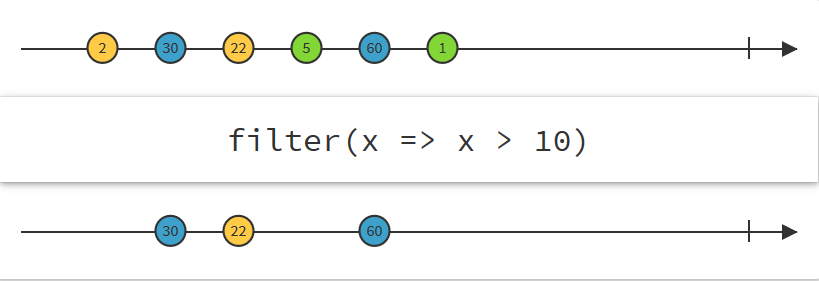
\includegraphics[width=1\textwidth]{Abb/filter}
	\caption{Datenfluss Filter-Operation}
	\label{pic:filter}
\end{figure}
Wie der Name schon sagt, handelt es sich bei Filter um eine Operation die einen Ausdruck prüft, und sofern das Element gültig ist, wird es weitergeben. Verwendet wir hier der von RxJava mitgebrachte Datentyp \textit{Predicate}. Er beinhaltet eine Methode \textit{test()} welche ein boolean zurück liefert. Somit ist es möglich einfache aber auch komplexere Überprüfungen innerhalb der Filter-Operation auszuführen. Im Bild \ref{pic:filter} sieht man eine Filterung nach dem Kriterium, dass nur jeden Element, das eine Wert größer 10 inne hält, ausgegeben wird. Da jedes Element sequentiell überprüft wird, erhält das untere Observable immer genau dann ein Element wenn es auch zu diesem Zeitpunkt die Prüfung passiert hat. In Java-Code sieht das ganze dann aus wie in Listing \ref{lst:filterop}. Innerhalb des Predicate wird die \textit{test()}-Methode überschrieben und die Prüfung ob der Wert größer 10 ist durchgeführt. 
\lstinputlisting[linerange={13-22}, caption={Beispiel Filter Operation}, label=lst:filterop]{../SystemMonitor/examples/operators/Ops.java} 
Parametriert wird das Predicate auf ein den Wert Integer, da nur ein Datentyp übergeben wird, Resultat is immer Datentyp boolean. Das Predicate kann natürlich auch inline und anonym deklariert werden.
\subsection{Operation map()}
Die Map-Operation gilt als Transformationsoperation. Ihre Aufgabe ist es, jeden auftretenden Wert auf eine Funktion abzubilden und das Resultat auszugeben. In Abbildung \ref{pic:map} sieht man auf dem ursprünglichen Observable drei auftretenden Elemente. Jedes dieser Elemente wird mit 10 multipliziert und danach auf das resultierenden Observable ausgegeben. 
\begin{figure}
	\centering
	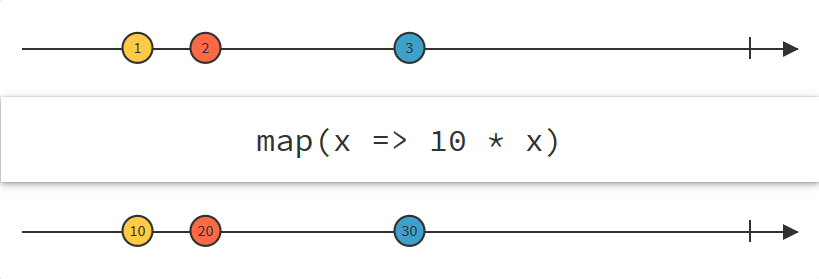
\includegraphics[width=1\textwidth]{Abb/map}
	\caption{Datenfluss Map-Operation}
	\label{pic:map}
\end{figure}
\lstinputlisting[linerange={25-26}, caption={Beispiel Map Operation}, label=lst:mapop]{../SystemMonitor/examples/operators/Ops.java} 
In Programmcode wird es wie erwartet als Lambda-Ausdruck dargestellt. Innerhalb des Mapping wird $x -> x \cdot 10$ abgebildet.
\subsection{Operation merge()}
Merge repräsentiert eine Observable-Komposition. Es handelt sich hierbei um eine recht einfache Variante, denn es werden lediglich alle Elemente aus mindestens zwei Observables in einen Observable-Stream zusammengefasst. 
\begin{figure}
	\centering
	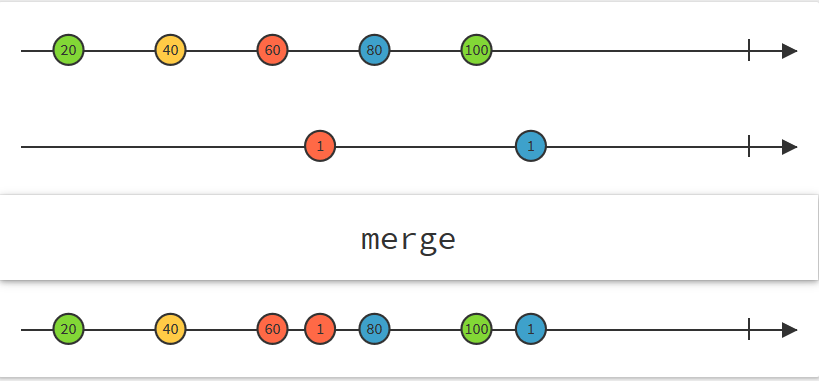
\includegraphics[width=1\textwidth]{Abb/merge}
	\caption{Datenfluss Merge-Operation}
	\label{pic:merge}
\end{figure}
Betrachtet man auch hier die passende Abbildung \ref{pic:merge} wird deutlich wie die Komposition stattfindet. Zu jedem Zeitpunkt eines der Observables ein Element ausgibt wird es an das zusammengeführte Observable weitergegeben. Somit wird die Reihenfolge der Elemente rein von dem Faktor Zeit bestimmt.
\lstinputlisting[linerange={34-36}, caption={Beispiel Merge Operation}, label=lst:mergeop]{../SystemMonitor/examples/operators/Ops.java} 
Im Listing \ref{lst:mergeop} ist die entsprechende Implementierung zu erkennen. Eines der Observables beinhaltet die Werte in zwanziger Schritten, das weitere produziert jede Nanosekunde ein Element. Das Mapping muss stattfinden, da immer nur Elemente eines Datentyps in ein Observable zusammen geführt werden können. Dadurch dass das Intervall jede Nanosekunde Werte ausgibt und die Subscription erst in dem Moment endet, in welchem alle Observables abgeschlossen sind, handelt es sich in diesem Beispiel um ein unendliches Observable. Wie vorab schon erwähnt ist die Unendlichkeit immer mit Vorsicht zu genießen hinsichtlich der Verwertbarkeit des Observerables und der Performanz einer Anwendung.
\subsection{Operation zip()}
Bei dem \textit{zip}-Operator handelt es sich ebenfalls um eine Komposition von Observables. Wie die Funktionsweise eines Reißverschlusses werden die Elemente miteinander verbunden. Abbildung \ref{pic:zipop} erläutert diese Weise genauer. Die Elemente der beiden Observables sind unterschiedlichen Typs und werden zu unterschiedlichen Zeitpunkten ausgegeben. Zip geht nun so vor, dass ab dem Moment, ab welchem mehrere Observables zusammen gelegt werden, immer die nächsten Elemente miteinander verknüpft werden und als Resultat ein neuer beziehungsweise anderen Datentyp entstehen kann.
\begin{figure}
	\centering
	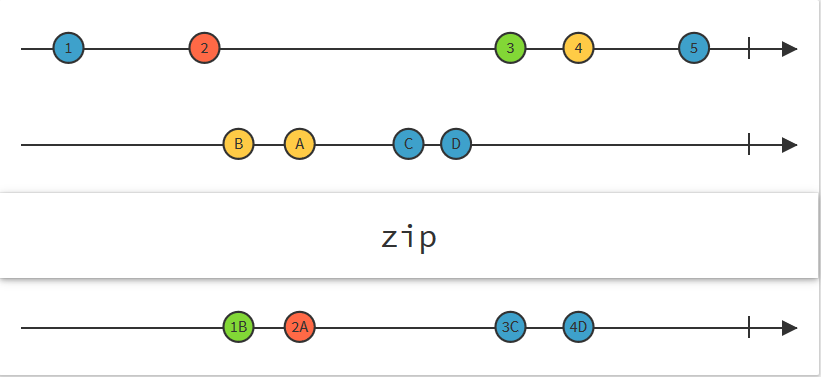
\includegraphics[width=1\textwidth]{Abb/zip}
	\caption{Datenfluss Zip-Operation}
	\label{pic:zipop}
\end{figure}
\lstinputlisting[linerange={29-31}, caption={Beispiel Zip Operation}, label=lst:zipop]{../SystemMonitor/examples/operators/Ops.java} 
Um es sich wieder von Entwicklungsseite zu veranschaulichen ist in Listing \ref{lst:zipop} ein einfaches Beispiel dargestellt. Wie in der Abbildung werden einmal Zahlen einmal Buchstaben als Observables repräsentiert und mit dem Zip-Operator verknüpft. Zip muss immer wissen, welche Objekte gezippt werden sollen, ebenso muss eine Funktion beschrieben werden, die definiert wie die Elemente miteinander verknüpft werden sollen. Hier ist wieder die Verwendung von Lambdas möglich, wie es auch im Listing stattfindet, oder es muss eine explizite Funktion definiert werden, als Objekt oder anonym. Auch hier ist wieder das Verhalten zu beachten, das erst eine Unsubscription stattfindet wenn alle verknüpften Streams beendet wurden. 